% !TeX root = scaffold-20.tex
\renewcommand{\imagepath}{../20-fermiqp/img}

\chapter{FermiQP: a Fermion Quantum Processor}
In this chapter, the FermiQP quantum gas microscopy experiment is introduced. It is first presented as a platform for quantum simulations and quantum computing. Then the projected experimental setup is outlined.

\section{A Versatile Microscope for Quantum Gases}\label{ch:quantum_gas_microscopy}
Within the last two decades, quantum gas microscopes have evolved into a well-proven and auspicious platform for exploring the diversity of phenomena in quantum many-body systems and for researching condensed matter physics. In these machines, neutral atoms are laser-cooled to sub-\si[]{\micro\kelvin} temperatures and arranged in regular patterns using optical lattices. Single-site imaging techniques allow resolving individual atoms and detecting their respective states~\cite{bloch_many-body_2008,gross_quantum_2017, gross_quantum_2021}, granting access to the physics of their interactions.

A key premise of these experimental explorations is that, rather than simulating quantum phenomena on classical computers using established models of physics, it is by far more advantageous to research them in controllable and isolated quantum systems~\cite{feynman_simulating_1982}. The main drawback of computer simulations that the size of the models and the computation time necessary to solve them scale exponentially with the extent of the described system.

While the first quantum gas microscopes in the late 2000s were based on bosonic rubidium (e.g.~\cite{sherson_single-atom-resolved_2010}), first results from experiments using fermionic alkali atoms were published in 2015, such as for potassium~\cite{cheuk_quantum-gas_2015} and lithium \cite{parsons_site-resolved_2015, omran_microscopic_2015}.

The FermiQP project, which was launched in 2021, is one of the newest fermion quantum gas microscopy experiments operated with lithium. It aims for surpassing existing fermionic lithium experiments with respect to precision, the number of trapped atoms, as well as coherence and atom lifetime. It will combine two modes of operation: In the so-called \textit{analog mode}, FermiQP will use the lithium atoms in optical lattices for investigating the nature of strongly interacting fermionic particles, which can be described by the Fermi-Hubbard model~\cite{hubbard_electron_1963, esslinger_fermi-hubbard_2010}. In the \textit{digital mode} on the other hand, FermiQP will act as a quantum computing platform exploiting the properties of its fermionic atoms and taking advantage of the long coherence times and the parallelizability of gate operations in optical lattices~\cite{zhang_functional_2022}. The key advantage over other platforms for quantum computing is the comparatively high scalability of quantum gases in optical lattices. The latter of both operation modes is what the experiment is named after: a \text{Fermion Quantum Processor}.

FermiQP is a consortium of many contributing institutes and scientific groups in different areas of physics across Germany. The actual quantum gas microscope, the \textit{FermiQP demonstrator}, is being built at the Max Planck Institute of Quantum Optics in Garching where this thesis was written.

The rest of this section introduces the techniques used in the FermiQP demonstrator and its projected features, followed by an overview of the planned experimental realization in the next section.

\subsection*{Laser Cooling}\label{ch:laser_cooling}
Cooling and trapping of atoms with laser light is the necessary first step for a quantum gas microscope to run. With the idea dating back to the 1970s~\cite{hansch_cooling_1975}, these techniques have paved the way for a whole realm of experiments exploring the world of atoms in ultracold regimes. After the 1997 nobel prize was awarded ``for development of methods to cool and trap atoms with laser light''~\cite{noauthor_nobel_nodate}, they have become a well-established technique employed in a multitude of quantum gas experiments, which themselves have led to the 2001 nobel prize for achieving Bose-Einstein condensation~\cite{noauthor_nobel_nodate-1}.

In the FermiQP demonstrator, different laser cooling techniques will be used: The atoms are first cooled and confined with a two- and a three-dimensional magneto-optical trap~\cite{foot_atomic_2005}, the latter of which is described in chapter~\ref{ch:mot}. Then gray molasses cooling~\cite{weidemuller_novel_1994} and evaporative cooling (see~\cite{foot_atomic_2005}, designed for FermiQP in~\cite{sun_construction_2022}), bring them into the \si[]{\micro\kelvin} regime.

\subsection*{Optical Lattices}\label{ch:optical_lattices}
Optical lattices are then used to confine the cooled atoms into individual sites arranged in regular patterns. These patterns are created by standing waves of high-power laser beams creating repeated dipole potential wells at points with high intensity. The spacing of these wells is half the wave length of the lattice laser light. Using multiple lattice beams, arbitrary lattice geometries can be implemented by varying the angle of the beams to each other and their respective phase and power. Figures~\ref{fig:2d_lattice} and~\ref{fig:1d_lattice} illustrate how optical lattices confine atoms in regular patterns. In order not to drive transitions in the atom, the laser is very far red-detuned~\cite{bloch_many-body_2008, bloch_quantum_2012}.

In the FermiQP demonstrator, multiple lattices are going to be used. Most notably the science lattice at \SI[]{1064}{\nano\meter} laser wave length providing the two-dimensional regular pattern that the atoms are positioned in for the experiments, and the deeper pinning lattice with less distance between the lattice sites, ensuring that the atoms are well-confined when imaging light is shone in. Raman sideband cooling will provide cooling for the atoms when they are confined in their lattice sites (see~\cite*{hilker_spin-resolved_2017}, designed for FermiQP in~\cite{krumm_notitle_2022}).

\begin{figure}
    \centering
    \begin{subfigure}[t]{0.3\textwidth}
        \centering
        \includegraphics[]{\imagepath/2d_lattice/2d_lattice.pdf}
        \caption{Visualization of a two-dimensional optical lattice with an atom in every site (image by Robin Groth)}
        \label{fig:2d_lattice}
    \end{subfigure}
    \hspace{0.03\textwidth}
    \begin{subfigure}[t]{0.3\textwidth}
        \centering
        \begin{tikzpicture}
            \begin{axis}[
                height=3.5cm,
                width=1.2\textwidth,
                xmin=-0.8, xmax=1.3,
                axis line style={draw=none},
                tick style={draw=none},
                xticklabels={,,}, yticklabels={,,}
            ]
                \addplot[thesisred, mark=none, line width=0.03cm, samples=500] {sin(2 * x*180)^2};
                \addplot[thesisgray, mark=*, only marks] coordinates {(-0.5, 0.2) (0.0, 0.2) (0.5, 0.2) (1.0, 0.2)};
            \end{axis}
        \end{tikzpicture}
        \caption{Optical lattice in one dimension}
        \label{fig:1d_lattice}
    \end{subfigure}
    \hspace{0.03\textwidth}
    \begin{subfigure}[t]{0.3\textwidth}
        \centering
        \begin{tikzpicture}
            \begin{axis}[
                height=3.5cm,
                width=1.2\textwidth,
                xmin=-0.8, xmax=1.3,
                axis line style={draw=none},
                tick style={draw=none},
                xticklabels={,,}, yticklabels={,,}
            ]
                \addplot[thesisred, mark=none, line width=0.03cm, samples=500] {0.5*sin(2 * x*180)^2 + 0.5*sin(x*180 + 45)^2};
                \addplot[thesisgray, mark=*, only marks] coordinates {(-0.45, 0.35) (-0.05, 0.35) (0.55, 0.35) (0.95, 0.35)};
            \end{axis}
        \end{tikzpicture}
        \caption{Example of an optical superlattice potential landscape in one dimension: Every other potential barrier is shallow, outlining an array of double-wells}
        \label{fig:1d_superlattice}
    \end{subfigure}
    \caption{Schematics of optical lattices}
    \label{fig:lattices}
\end{figure}

In FermiQP, the superlattice technique will be used: By overlapping an optical lattice with another lattice of double the lattice spacing, every other potential barrier between two sites can be lowered, creating an array of double-wells. By varying the phase and amplitude of the lattice beams, different barrier heights can be realized, allowing to control the tunneling rate between the sites of the double-well.

\subsection*{Imaging}
FermiQP will implement fluorescence imaging, meaning that light scattered by the atoms is used as an imaging signal, and absorption imaging, meaning that the absorption of light reveals the position of individual atoms in the lattice. Two objectives will be used for collecting the imaging signal. In addition to observing positions, spin states of the atoms can be read out using spin-resolving detection techniques, e.g.~by spatially separating atoms of different spin state into the two double-well sites~\cite{boll_spin-_2016} or into different layers perpendicular to the lattice plane~\cite{koepsell_robust_2020} with magnetic fields like in a Stern-Gerlach experiment. An example of spin-resolved imaging is shown in figure~\ref{fig:absorption_image}.

\begin{figure}
    \centering
    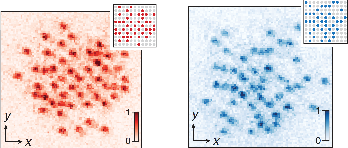
\includegraphics[]{\imagepath/imaging/imaging.pdf}
    \caption{Example of spin-resolving imaging (from~\cite{koepsell_robust_2020}): The two images show the position of spin-up and spin-down atoms in the lattice.}
    \label{fig:absorption_image}
\end{figure}

\subsection*{Quantum Simulations in the Analog Mode}\label{ch:analog_mode}
In the analog operation mode, the fermionic lithium atoms in the optical lattices are used for simulating phenomena of Fermi gases, such as the Mott-insulating and anti-ferromagnetic phases, as well as fermions paired to bosonic molecules, superfluidity and  superconductivity, and others~\cite{bloch_quantum_2012,esslinger_fermi-hubbard_2010}. These phases emerge as different domains in the Fermi-Hubbard Hamiltonian describing a system of fermions in the lowest energy band at lattice sites $i$ and $j$ with spin state $\nu \in \{\Ket{\uparrow}, \Ket{\downarrow}\}$~\cite{hubbard_electron_1963,esslinger_fermi-hubbard_2010}:
\begin{align}\label{eq:fermi_hubbard_hamiltonian}
    \hat H =
    \underbrace{-t \sum\limits_{\Braket{i,j}, \nu} \left(\hat a^\dagger_{i, \nu} \hat a_{j, \nu} + \text{h.c.}\right)}_\text{kinetic term/tunneling}
    + \underbrace{U \sum\limits_i \hat n_{i, \Ket{\uparrow}} \hat n_{i, \Ket{\downarrow}}}_\text{on-site interaction}
    + \underbrace{\sum\limits_{i, \nu} \epsilon_{i} \hat n_{i, \nu}}_\text{offset}
\end{align}
with $\Braket{i,j}$ meaning that $i$ and $j$ are neighboring sites. The first term describes the rate of tunneling of a particle between two neighboring sites with the creation operator $\hat a^\dagger$ and the annihilation operator $\hat a$. The tunneling $t$ can be set in optical lattice experiments by lowering the potential barrier between sites, as hinted at above, and reciprocally depends on the atomic mass implying comparatively high tunneling rates for the lightweight lithium atoms~\cite{jaksch_cold_1998}. The on-site interaction term describes the energy shift $U$ in sites where two atoms (in different spin states) are present, with $U > 0$ denoting repulsive and $U < 0$ denoting attractive interactions. The interaction between atoms on the same site depends on the s-wave scattering length $a$ and the atom mass $m$ as $U \propto \frac{a}{m}$. $a$ can be varied in the experiment using Feshbach resonances as outlined in the next paragraph. Finally, $\epsilon_i$ is a site-dependent potential offset~\cite{esslinger_fermi-hubbard_2010}.

\begin{figure}
    \centering
    \begin{tikzpicture}
            \begin{axis}[
                height=3.5cm,
                width=0.8\textwidth,
                xmin=-0.8, xmax=1.35,
                axis line style={draw=none},
                tick style={draw=none},
                xticklabels={,,}, yticklabels={,,}
            ]
                \addplot[color=thesisred, mark=none, line width=0.06cm, samples=500] {sin(2 * x*180)^2};

                \addplot[color=thesisred, mark=*, mark size=0.14cm, only marks] coordinates {(-0.5, 0.2)};
                \addplot[color=thesisred, opacity=0.5, mark=*, mark size=0.14cm, only marks] coordinates {(0.0, 0.2)};

                \draw[yscale=1, ->] (axis cs:-0.5, 0.30) arc [radius=0.25, start angle=180, delta angle=90, end angle=0]; 
                \draw (axis cs: -0.25, 0.65) node {\small $t$};

                \addplot[color=thesisred, mark=*, mark size=0.14cm, only marks] coordinates {(1.0-0.05, 0.7)};
                \addplot[color=thesisblue, mark=*, mark size=0.14cm, only marks] coordinates {(1.0+0.05, 0.7)}; 
                \draw[<->] (1.25, 0.22) -- (1.25, 0.68) node[midway, right] {\small $U$};

                \draw[color=thesisgray, thin, dashed] (0.05, 0.2) --(1.25, 0.2);
                \draw[color=thesisgray, thin, dashed] (1.1, 0.7) --(1.25, 0.7);
            \end{axis}
    \end{tikzpicture}
    \caption{Tunneling and on-site interactions in the Fermi-Hubbard Hamiltonian~\eqref{eq:fermi_hubbard_hamiltonian} in an optical lattice~\cite{esslinger_fermi-hubbard_2010}: The tunneling of a particle is determined by $t$, whereas the on-site interaction energy $U$ is the energy sites with two particles (of different spin state) are shifted by.}
    \label{fig:fermi_hubbard_schematic}
\end{figure}

\paragraph*{Feshbach Resonances} Feshbach resonances allow varying the scattering length $a$ of certain atoms by applying a constant magnetic field and so also the on-site interaction $U$ in the Fermi-Hubbard model. In the collision process of two atoms, this magnetic field sets the energy difference between two states of the atoms, a scattering state and a bound molecular state with different magnetic moments. At a certain magnetic field $B_0$, these energy levels coincide and the scattering length becomes infinite, which is a Feshbach resonance. For $B < B_0$, the scattering length is positive, $a > 0$, and $U$ is repulsive, whereas for $B > B_0$, one gets $a < 0$ and attractive $U$:
\begin{align}
    a = a_\text{background} \left(1 - \frac{\Delta}{B-B_0}\right)
\end{align}
with the width $\Delta$ of the Feshbach resonance and the background scattering length $a_\text{background}$ at the absence of a magnetic field. Fermionic lithium has a broad ($\Delta = \SI[]{300}{\gauss}$) resonance at $B_0 = \SI[]{834}{\gauss}$~\cite{chin_feshbach_2010}, allowing a large variation of the on-site interaction in the FermiQP demonstrator experiment via adjustable magnetic fields up to \SI[]{1200}{\gauss}.

\subsection*{Quantum Computing in the Digital Mode}\label{ch:digital_mode}
In the digital mode, FermiQP aims to serve as a platform for universal quantum computing. Quantum computers are supposed to accelerate the execution of certain algorithms that scale exponentially with problem size on classical computer hardware in terms of their execution time, such are Shor's algorithm for factoring large numbers~\cite{shor_algorithms_1994}\todo{not precise enough?}. For this they make use of entanglement and superposition of states to achieve this speed-up. In quantum computers, the smallest unit of information is a so-called qubit, a two-level system of quantum states~\cite{nielsen_quantum_2010, hidary_quantum_2021, ladd_quantum_2010, mainzer_quantencomputer_2020}.

In the FermiQP demonstrator, qubits are encoded in the two energetically lowest hyperfine magnetic sublevels of the $2\text{s}^2\text{S}_{1/2}$ manifold, called $\Ket{1}$ and $\Ket{2}$. In the domain of high magnetic fields of \SIrange[]{500}{1000}{\gauss}, the magnetic sublevels of this manifold are separated by multiple \si[]{\giga\hertz}.\cite{gehm_properties_2003,wei_magnetic-field_2013}.

Universal quantum computers need to implement two kinds of gate operations: single-qubit gates for flipping indivudial qubits and two-qubit gates for entangling pairs of qubits~\cite{hidary_quantum_2021, mainzer_quantencomputer_2020}:\todo{more citations}

\paragraph*{Single-Qubit Gates}
Single-qubit gates in the FermiQP demonstrator are implemented with Raman transitions driven by an ultraviolet tweezer beam at \SI[]{323}{\nano\meter} allowing addressing single individual sites of the optical lattice. Due to its low mass, Raman transitions on the manifold between the two aforementioned qubit states are highly suppressed in  ferimonic lithium~\cite{wei_magnetic-field_2013}. In the FermiQP demonstrator, transitions between the two qubit states are therefore implemented with a detour over the magnetic sublevel $\Ket{6}$ via global microwave and radio-frequency pulses, as explained in figure~\ref{fig:single_qubit_gates}.

\begin{figure}
    \centering
    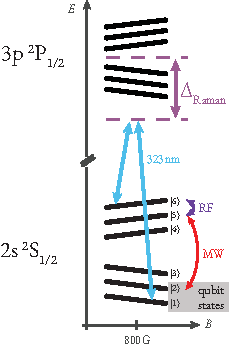
\includegraphics[]{\imagepath/single_qubit_gates/single_qubit_gates.pdf}
    \caption{Single qubit gate scheme in the FermiQP demonstrator (figure by Robin Groth): The states $\Ket{1}$ and $\Ket{2}$ in the the $2\text{s} ^2\text{S}_{1/2}$ manifold constitute a qubit.
    \SI[]{323}{\nano\meter} addressing beams couple $\Ket{1}$ with $\Ket{6}$ by a Raman transition via the $3\text{p} ^2\text{P}_{1/2}$ manifold. This Raman coupling can be driven selectively by focusing the \SI[]{323}{\nano\meter} beam onto individual sites of the optical lattice.
    A combination of a microwave (MW) and a radio-frequency (RF) pulse applied on all lattice sites couples $\Ket{2}$ and $\Ket{6}$ via $\Ket{5}$.\\
    A single qubit gate operation consists of an MW-RF pulse combination, then the Raman addressing, and another MW-RF pulse combination.
    In the addressed qubit, $\Ket{1}$ is coupled with $\Ket{6}$ via the Raman transition, which then is coupled to $\Ket{2}$ by the MW-RF pulses; $\Ket{2}$, on the other hand, is coupled by the MW-RF pulses to $\Ket{6}$, and then to $\Ket{1}$ via the Raman transition.
    All qubits that are not addressed by the Raman beam are preserved: The two MW-RF pulse combinations bring the $\Ket{2}$ qubits back to their original state while leaving the $\Ket{1}$ qubits unaffected.}
    \label{fig:single_qubit_gates}
\end{figure}

\paragraph*{Two-Qubit Gates}
Two-qubit operations in the FermiQP demonstrator will be implemented with collisional gates in double-wells of the superlattice. There two atoms are entangled by lowering the potential barrier and allowing interaction between them. While the idea of two-qubit gates in optical lattices dates back more than two decades~\cite{jaksch_fast_2000, anderlini_controlled_2006,trotzky_time-resolved_2008}, collisional gates have recently gained interest with quantum computing in optical lattices entering the realm of possibility~\cite{dai_generation_2016, yang_cooling_2020, zhang_functional_2022}.\todo{check and improve citations}

Arbitrary pairs of atoms can be entangled by moving them into neighboring lattice sites in the double-wells in the superlattice with optical tweezers, and then lowering the double-well barriers such that the atoms interact and entanglement is created, as depicted in figure~\ref{fig:two_qubit_gates}. These two-qubit gate operations can be conducted for multiple pairs of atoms in parallel by using multiple tweezers. Lowering the potential barrier is a global operation, hence all pairs of atoms in double-wells are entangled at the same time.

\begin{figure}
    \centering
    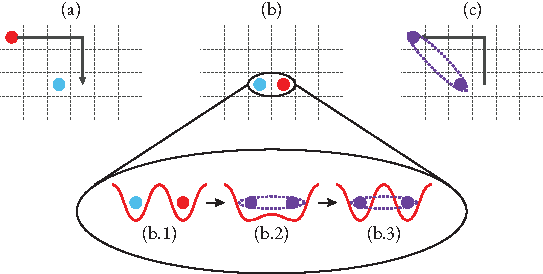
\includegraphics[]{\imagepath/two_qubit_gates/two_qubit_gates.pdf}
    \caption{Two-qubit collisional gate scheme in the FermiQP demonstrator: a: Two atoms that are supposed to be entangled are moved into neighboring sites using optical tweezers. b: The atoms are entangled by lowering the potential barrier in the double well (b.2) and letting the atoms interact. When the potential barrier is ramped up again, the entanglement (purple ellipse) is preserved. c: Then the atoms are moved to their original positions with the entanglement preserved.}
    \label{fig:two_qubit_gates}
\end{figure}

\null

In the next section, the planned experimental implementation of the FermiQP demonstrator will be outlined.



\section{Experimental Setup of the FermiQP Demonstrator}
The fermionic lithium atoms in the FermiQP demonstrator are prepared under ultra-high vacuum conditions and trapped in the optical lattices in a glass cell. The vacuum chamber and all adjacent features of the experiment are illustrated in figure~\ref{fig:chamber} and explained in the following.

\begin{figure}
    \centering
    \begin{subfigure}[t]{0.64\textwidth}
        \centering
        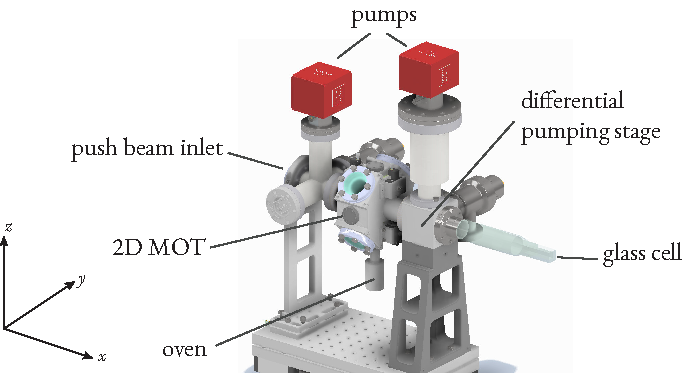
\includegraphics[width=\linewidth]{\imagepath/chamber/chamber_side_0.pdf}
        \caption{Drawing of the vacuum chamber with the glass cell}
        \label{fig:chamber_coarse}
    \end{subfigure}
    \begin{subfigure}[t]{0.34\textwidth}
        \centering
        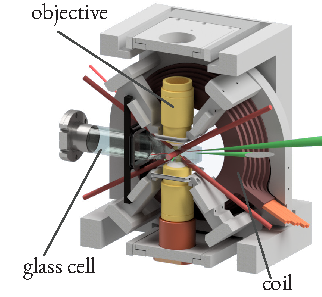
\includegraphics[width=\linewidth]{\imagepath/chamber/chamber_detail_0.pdf}
        \caption{Detail view of the glass cell and its surroundings}
        \label{fig:chamber_detail}
    \end{subfigure}
    \caption{Drawing of the planned design of the vacuum chamber: Atoms are evaporated from the oven into the chamber of the two-dimensional magneto-optical trap (2D MOT) where the atoms are confined to a one-dimensional cloud. This cloud of atoms is then push along the $x$ axis through the differential pumping stage into the ultra-high vacuum region. There they reach the glass cell where they are captured by the three-dimensional magneto-optical trap. The objectives for imaging sit above and below the glass cell, the coils for creating magnetic fields and gradients sit on the sides, held by a massive metal cube. Some exemplary lattice laser beams shone into the glass cell are shown in the detail view (red and green tubes). The axes are aligned such that the atomic beam towards the glass cell runs along the $x$ axis, the $z$ axis points to the left as seen from the atomic beam, the $y$ axis points upwards.}  
    \label{fig:chamber}
\end{figure}

\paragraph{Vacuum System}
The vacuum system of the FermiQP demonstrator experiment consists of two sections: the high vacuum oven section with pressures down to \SI[]{e-10}{\milli\bar} and the ultra-high vacuum science section down to \SI[]{5e-12}{\milli\bar} where the atoms are kept in a cuboid-shaped uncoated glass cell  with $\SI[]{12}{\milli\meter} \times \SI[]{12}{\milli\meter}$ inner cross-section. The low pressure there avoids collisions with other particles and so guarantees long coherence times. The vacuum is maintained by two ion getter pumps atop the chamber. The two sections are connected with a thin differential pumping tube with low conductivity impeding the flow of residual gas in the high vacuum to the ultra-high vacuum section, still allowing a beam of atoms to pass through.

\paragraph{Cooling Cycle}
The fermionic lithium atoms are evaporated from chunks of lithium in the oven located in the lower part of the high vacuum part. Atop the oven, they reach the two-dimensional magneto-optical trap where they are confined to a thread-like atomic filament along the $x$ axis~\cite{qesja_design_2022}.  A push beam along this axis gives them momentum such that they fly through the differential pumping tube into the ultra-high vacuum section to the glass cell. Using a two-dimensional magneto-optical trap makes the vacuum chamber very compact and small compared to setup with a Zeeman slower, still providing the necessary flux rate and quality of the atomic beam~\cite{tiecke_high-flux_2009}.

At the glass cell, the atoms are captured in a three-dimensional magneto-optical trap which was designed in the scope of this thesis (chapter~\ref{ch:mot}). The atoms are then further cooled down with the gray molasses technique (also in chapter~\ref{ch:mot}) and evaporative cooling in an optical dipole trap~\cite{sun_construction_2022} such that they can be loaded into the optical lattices.

\paragraph{Lasers}
The FermiQP demonstrator uses a multitude of laser frequencies, most notably the near-resonant \SI[]{671}{\nano\meter} light for cooling the atoms in the magneto-optical traps, the gray molasses, and during Raman sideband cooling in the optical lattice, far off-resonant \SI[]{1064}{\nano\meter} and \SI[]{1070}{\nano\meter}  light for optical trapping in the optical dipole trap and the optical lattices, as well as \SI[]{323}{\nano\meter} light for Raman addressing.

\paragraph{Imaging}
Imaging signals are collected by two objectives, one for visible and one for ultraviolet light, sitting below and above the glass cell. During imaging, the atoms caught in the optical lattices can be pinned down by a deep and narrow-spaced pinning lattice such that incident imaging light doesn't push them out of their positions.

\paragraph{Magnetic Fields}
The magnetic fields for the three-dimensional magneto-optical trap and the Feshbach fields are created by coils sitting left and right of the glass cell. They were developed and characterized during this thesis (in chapter~\ref{ch:coils}). In addition to that, compensation coils around the experiment table provide arbitrary offset fields of up to \SI[]{3}{\gauss} at the position of the trapped atoms.

\null

In the next chapter, the theory of magneto-optical traps and the projected implementation of the three-dimensional magneto-optical trap in the FermiQP demonstrator will be presented in detail.